\documentclass[a4paper]{article}
\usepackage[utf8]{inputenc}

\usepackage{graphicx}  % import graphics
\usepackage{listings}  % support source code listing
\usepackage{amsmath}  % math stuff
\usepackage{amssymb} % 
\usepackage{a4wide} % wide pages
\usepackage{fancyhdr} % nice headers
\usepackage{tikz}
\usetikzlibrary{arrows}
\usetikzlibrary{petri}

\lstset{basicstyle=\footnotesize,language=Python,numbers=left, numberstyle=\tiny, stepnumber=5,firstnumber=0, numbersep=5pt} % set up listings
\pagestyle{fancy}             % header

\usepackage[none]{hyphenat}
\sloppy

% change enums style: first level (a), (b), (c)           
\renewcommand{\labelenumi}{\arabic{enumi}.}
\renewcommand{\labelenumii}{\alph{enumii})}

%term/semester
\newcommand{\term}{
	Summer 2012 -- Saarland University
} 

%lecture name
\newcommand{\lecture}{
	Algorithm Engineering
}           

%assignment iteration
\newcommand{\assignment}{
	Team FortyTwo Final Report
}

%set up names, matricle number, and email
\newcommand{\authors}{
  Florian Benz, Steven Schäfer, Bernhard Schommer
}

% use to start a new exercise
\newcommand{\exercise}[1]
{
  \stepcounter{subsection}
  \subsection*{Exercise \thesubsection: #1}

}

\begin{document}
\title{
  \vspace{-3cm}
  \large
  \lecture \\
  \small \term \\
  \huge \assignment
}
\author{\small \authors}

\setlength \headheight{25pt}
\fancyhead[R]{\begin{tabular}{r}\lecture \\ \assignment \end{tabular}}
\fancyhead[L]{\authors}

\maketitle

\section{Overview}

\subsection{Pre-processing}

First, we pre-process the OSM data to extract a single street graph consisting of intersections in the original graph.
For each travel mode, we extract whether a vertex or an edge is accessible.
Our graph format consists of a compressed sparse row representation of the graph.
Each vertex and edge can be uniquely identified by its offset.
We use this to store additional attributes like distance, steps and positions in separate files.

The second step of the pre-processing partitions the large graph into small clusters with 
nearly the same amount of vertices.
We employ Metis~\cite{met12} for the graph partitioning with the objective of minimizing
the number of edges between clusters.
After this step, we have several clusters (e.g. 1000) and one overlay graph that consits
of all boundary vertices and the cut edges.
The result for Europe is shown in Figure~\ref{fig}.

\begin{figure}
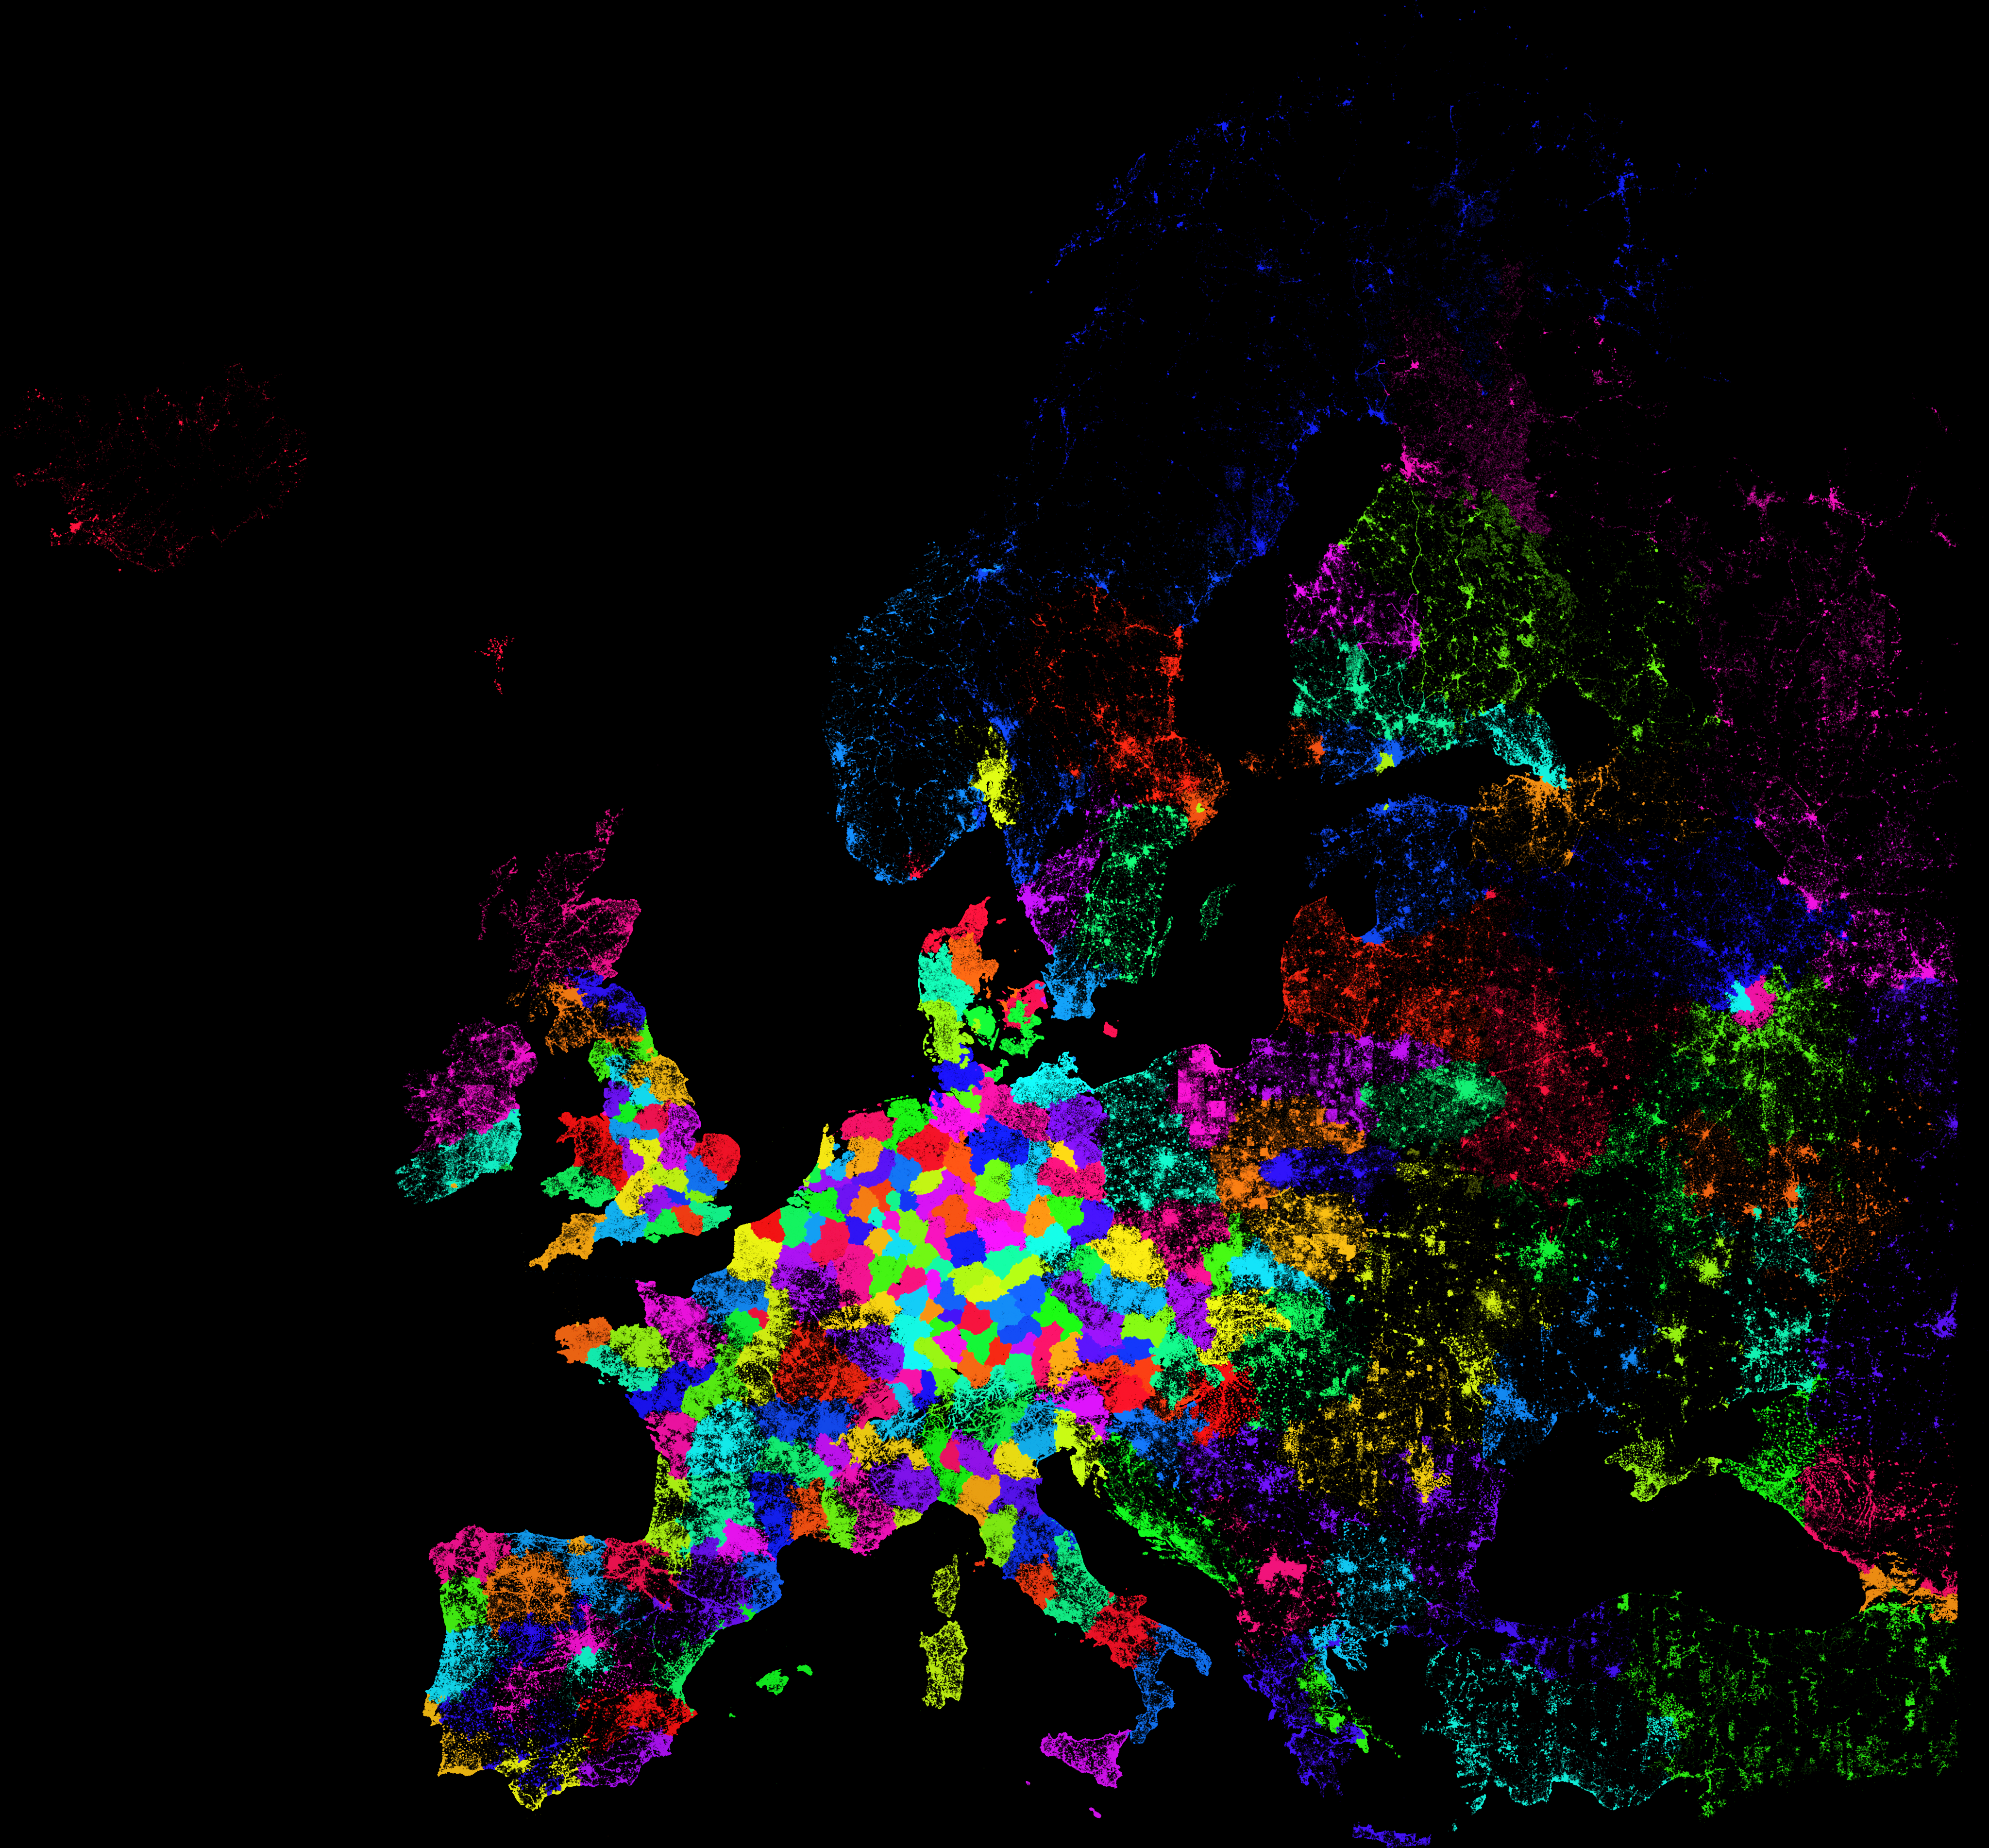
\includegraphics[scale=0.1]{terminal}
\caption{The street graph of Europe partitioned into balanced clusters}
\label{fig}
\end{figure}

Up to now, the pre-processing is independent of the used metrics.
This has the advantage that only the metric-specific pre-processing is needed
for changes or additional metrics.
For each cluster, metric, and transport mode, we pre-compute a matrix of the shortest
paths of all boundary vertices to all other boundary vertices of the cluster.

The whole idea of metric-independent partitioning and the metric matrices is based
on the approach presented by Delling et al~\cite{del11}.
This is the approach used for Microsoft Bing.
However, the idea is not new. 
The earlier benchmarks by Schütz~\cite{sch04} show that a good partitioning leads
to better performance. Especially in contrast to a simple grid.

One advantage of the partition-based approach is that in contrast to many other 
approaches arbitrary metrics  are supported and take advantage of fast queries.
Another advantage of the separated pre-processing steps is that updates can 
be made so fast that real-time traffic updates are possible. 

\subsection{Queries}

During the startup of the server, all files are mapped into the server's address space.
As a result our startup overhead is negligible and we do not have to load data from disk afterwards.

When a query arrives, we find for each waypoint the nearest node in the OSM data.
This might not correspond to a vertex in our street graph;
in this case the node lies on an edge and we compute all reachable endpoints of this edge.
At this point, we run Dijkstra's algorithm in both clusters and
a bidirectional version of Dijkstra's algorithm on the overlay graph.
Finally, the resulting JSON object is created and returned.

The street graph is significantly smaller than the original OSM graph.
Furthermore, it is sparse; the average out-degree is around 2.4.
To improve the efficiency of Dijkstra's algorithm on street graphs, we use a 4-heap
that is optimized for the memory characteristics on the server.

To find the nearest neighbor, we use precomputed k-d trees.
This results in very fast queries during runtime.
The construction algorithm is reminiscent of quicksort.
On disk the k-d tree is stored as a permutation of encoded vertex indices, edge offset, and step offsets.
A k-d tree is created for each cluster and for the overlay graph.
To find the matching cluster for a waypoint, we use precomputed bounding boxes.

We use Go as our implementation language.
Go is a modern, concurrent and statically compiled programming language.
As the standard library comes with an HTTP server and JSON marshaling,
the initial implementation went very smoothly.
In addition, it is a joy to parallelize computations.

\section{Encountered Problems}

The OSM data turned out to be astonishingly clean, compared to the output of a monkey with a typewriter.
By default the data is sorted by creation date, which is nice if you want to build a history viewer.
For our purposes, this ordering is useless if you want to apply any kind of graph algorithm
directly to the OSM files.

Due to the Go garbage collector, the addressable memory on a 64 bit machine is limited to 16 GB.
Our parser needs more memory to process the whole of Germany for pedestrian routing.
This is solved by allocating large data structures in the non-GC heap
and in addition we reduced our memory footprint.

\section{Additional Features}

Our server can perform concurrent non-blocking logging with accurate timing information.
In addition, the server can output profiling data for a request;
this has already been useful in troubleshooting performance problems.

Additionally, we have created a small JavaScript based frontend that 
gives us an easy way to test and visualize the results of our implementation
(see http://urania.mpi-inf.mpg.de:23401/awesome).
As a reference route, the result of Google Directions is shown side-by-side.
Google Places autocompelte is included for convenience.

\begin{thebibliography}{9}
  
\bibitem{del11}
	D. Delling, A. V. Goldberg, T. Pajor, R. F. Werneck, \emph{Customizable route planning}. SEA'11. 
	
\bibitem{met12}
    \emph{Metis}, http://glaros.dtc.umn.edu/gkhome/metis/metis/overview.

\bibitem{sch04}
	B. Schütz, \emph{Partition-Based Speed-Up of Dijkstra's Algorithm}. 2004, http://citeseerx.ist.psu.edu/viewdoc/summary?doi=10.1.1.115.3514.

\end{thebibliography}

\end{document}
